\documentclass[11pt]{article}
\usepackage[margin=1in]{geometry}
\usepackage{amsmath,amssymb,booktabs,array,longtable}
\usepackage{graphicx}
\graphicspath{{figures/}}
\usepackage{hyperref}
\usepackage{enumitem}
\usepackage{titlesec}
\usepackage{float}
\usepackage{caption}
\usepackage{mathtools}
\usepackage{setspace}

\onehalfspacing

\begin{document}

\begin{center}
{\LARGE\textbf{Shiv Nadar University Chennai}}\\[4mm]
\end{center}

\renewcommand{\arraystretch}{1.6}
\setlength{\tabcolsep}{10pt}

\begin{center}
\begin{tabular}{|p{4cm}|p{9.5cm}|}
\hline
\textbf{Degree \& Branch} & B.Tech Artificial Intelligence \& Data Science, Semester V \\ \hline
\textbf{Subject} & CS3807 -- Deep Learning Laboratory \\ \hline
\textbf{Name} & Madhav.S \\ \hline
\textbf{Section} & AIDS `B' \\ \hline
\textbf{Register Number} & 24011101066 \\ \hline
\end{tabular}
\end{center}

\vspace{5mm}

\begin{center}
{\Large\textbf{Experiment 4}}\\[1mm]
{\large\textbf{Comparative Study of Deep Convolutional Neural Network Architectures Using Transfer Learning}}
\end{center}

\vspace{4mm}

%----------------------------------------------------------

\section*{1. Objective}

\begin{itemize}[leftmargin=*]
\item Study the evolution of deep CNN architectures.
\item Compare LeNet-5, AlexNet, VGG16, GoogleNet and ResNet.
\item Understand transfer learning.
\item Fine-tune a pretrained CNN model.
\item Compare classification performance before and after fine-tuning.
\end{itemize}

%----------------------------------------------------------

\section*{2. Introduction}

Deep Convolutional Neural Networks have become the dominant models for computer vision because they automatically learn hierarchical features from images, rather than relying on handcrafted feature extraction. The evolution of CNN architectures has consistently focused on improving classification accuracy while reducing computational complexity and training difficulty.

The progression began with LeNet-5 and evolved through AlexNet, VGGNet, GoogleNet, and ResNet, each introducing an innovation that meaningfully improved image classification performance.

%----------------------------------------------------------

\section*{3. Evolution of CNN Architectures}

\begin{table}[H]
\centering
\caption{Evolution of Deep CNN Architectures}
\begin{tabular}{lcp{7cm}}
\toprule
Model & Year & Major Contribution \\
\midrule
LeNet-5 & 1998 & First practical convolutional neural network \\
AlexNet & 2012 & ReLU activation, Dropout, and GPU training \\
VGG16 & 2014 & Uniform $3\times3$ convolution filters \\
GoogleNet & 2014 & Inception modules for multi-scale feature extraction \\
ResNet & 2015 & Residual learning using skip connections \\
\bottomrule
\end{tabular}
\end{table}

\subsection*{LeNet-5}
Proposed by Yann LeCun in 1998 for handwritten digit recognition. Consists of two convolution layers, two average pooling layers, and fully connected layers. Demonstrated that convolutional networks could automatically learn image features without handcrafted feature extraction.\\
\textbf{Advantages:} small number of parameters, fast training, suitable for OCR.

\subsection*{AlexNet}
Won the 2012 ImageNet Challenge by a large margin, reducing the classification error significantly. Introduced ReLU activation, Dropout regularization, and GPU-based training.\\
\textbf{Major innovations:} ReLU activation, Dropout, GPU implementation, data augmentation.

\subsection*{VGG16}
Demonstrated that stacking multiple small $3\times3$ convolution filters could outperform larger filters while increasing network depth.\\
\textbf{Advantages:} excellent feature extraction, simple architecture, high classification accuracy.

\subsection*{GoogleNet (Inception Network)}
Proposed by Szegedy et al. in 2014. Introduced the \textbf{Inception module}, which performs multiple convolution operations in parallel using different filter sizes -- $1\times1$, $3\times3$, $5\times5$ convolutions and max pooling applied simultaneously, with the outputs concatenated to obtain multi-scale feature representations. The use of $1\times1$ convolutions before larger kernels reduces the number of trainable parameters and computational complexity.\\
\textbf{Advantages:} multi-scale feature extraction, fewer parameters than VGG16, high computational efficiency, better classification performance.

\subsection*{ResNet}
Increasing CNN depth often causes the vanishing gradient problem, making optimization difficult. ResNet solves this using skip (residual) connections, allowing gradients to flow directly through the network. Instead of learning $H(x)$, ResNet learns the residual $F(x) = H(x) - x$, so that:
\[
\text{Output} = F(x) + x
\]
where $F(x)$ is the residual mapping and $x$ is the identity mapping.\\
\textbf{Advantages:} eliminates vanishing gradients, enables very deep networks, faster convergence, high ImageNet accuracy.

\begin{table}[H]
\centering
\caption{Comparison of Architectures (Literature Reference Values)}
\begin{tabular}{lccp{4.5cm}}
\toprule
Architecture & Depth & Parameters & Main Contribution \\
\midrule
LeNet-5 & 7 & 60K & First CNN \\
AlexNet & 8 & 61M & ReLU + Dropout \\
VGG16 & 16 & 138M & Deep $3\times3$ filters \\
GoogleNet & 22 & 6.8M & Inception Modules \\
ResNet50 & 50 & 25.6M & Residual Learning \\
\bottomrule
\end{tabular}
\end{table}

\textit{Note: these are the standard published parameter counts for the original ImageNet-classification versions of each architecture, included here for architectural context. This experiment implements and trains only VGG16 via transfer learning, per Task 2's instruction to select one pretrained model -- the other four architectures are discussed conceptually above but not separately trained here.}

%----------------------------------------------------------

\section*{4. Dilated Convolution}

Dilated (atrous) convolution increases the receptive field of a kernel without increasing the number of parameters. The dilation rate $D$ controls the spacing between kernel elements: a standard convolution has $D=1$, while a dilated convolution has $D>1$, spreading the same kernel weights over a wider area of the input.

\textbf{Applications:} semantic segmentation, medical image analysis, satellite imagery, object localization.

A quick sanity check confirms the mechanics: a $3\times3$ kernel with `dilation\_rate=2` applied to a $16\times16\times1$ input still produces an output of the same spatial size (with `'same'` padding), but its 9 weights now span a $5\times5$ area of the input instead of the usual $3\times3$ -- more context, same parameter count.

%----------------------------------------------------------

\section*{5. Transpose Convolution}

Transpose convolution (sometimes called deconvolution) performs \textbf{learnable upsampling} -- it increases the spatial dimensions of a feature map, the opposite of what pooling does. Unlike simple interpolation, the upsampling weights are learned during training.

\textbf{Applications:} image super-resolution, autoencoders, GANs, image generation, semantic segmentation (decoder path).

A stride-2 `Conv2DTranspose` layer applied to an $8\times8\times16$ feature map doubles its spatial resolution to $16\times16$, learning how to fill in the new pixels rather than simply repeating or interpolating existing ones.

%----------------------------------------------------------

\section*{6. Transfer Learning}

Transfer learning reuses a CNN that has already learned general-purpose visual features from a large dataset (typically ImageNet), instead of training a new network from scratch.

\textbf{Workflow:}
\begin{enumerate}[leftmargin=*]
\item Load a pretrained model with ImageNet weights.
\item Remove the original classifier.
\item Freeze the convolutional base.
\item Add new Dense layers suited to the new task.
\item Train the new classifier head.
\item Fine-tune selected convolutional layers.
\end{enumerate}

\textbf{Advantages:} faster convergence, higher accuracy on small datasets, reduced training time, lower computational cost.

%----------------------------------------------------------

\section*{7. Dataset}

\textbf{Dataset:} CIFAR-10\\
\textbf{Source:} Loaded directly via \texttt{tensorflow.keras.datasets.cifar10}

\begin{table}[H]
\centering
\caption{Dataset Summary}
\begin{tabular}{ll}
\toprule
Training Images & 50,000 \\
Testing Images & 10,000 \\
Number of Classes & 10 \\
Image Size & $32\times32\times3$ \\
Classes & Airplane, Automobile, Bird, Cat, Deer, Dog, Frog, Horse, Ship, Truck \\
\bottomrule
\end{tabular}
\end{table}

%----------------------------------------------------------

\section*{8. Experimental Procedure}

\subsection*{Task 1 -- Dataset Preparation}
CIFAR-10 was loaded via the Keras dataset API. Pixel values were normalized to the $[0,1]$ range, ten sample images were displayed (one per class), and the dimensions of the training and testing sets were printed and verified.

\subsection*{Task 2 -- Transfer Learning}
VGG16 was loaded with pretrained ImageNet weights, excluding its original 1000-class classifier. The convolutional base was frozen, and a new head was attached: Global Average Pooling $\rightarrow$ Dense(256, ReLU) $\rightarrow$ Dropout $\rightarrow$ Dense(10, Softmax).

\subsection*{Task 3 -- Model Training}
The model was trained with the Adam optimizer (learning rate $0.001$), batch size 32, categorical cross-entropy loss, and accuracy as the evaluation metric, for up to 15 epochs (within the specified 10--20 range), with early stopping on validation loss.

\subsection*{Task 4 -- Fine-Tuning}
The last convolutional block of VGG16 (\texttt{block5}) was unfrozen and trained for a further 8 epochs at a much lower learning rate ($1\times10^{-5}$), and classification accuracy was compared directly before and after fine-tuning.

\subsection*{Task 5 -- Model Evaluation}
The fine-tuned model was evaluated on the 10,000-image test set using accuracy, precision, recall, F1-score, a full classification report, and a confusion matrix.

%----------------------------------------------------------

\section*{9. Source Code}

The complete implementation, exactly as run in Colab, is hosted on GitHub.

\begin{center}
\url{https://github.com/smadhav2024/Deep_Learning_Lab/tree/main/Lab%204}
\end{center}

The repository contains the full notebook, the requirements needed to run it, and this report's LaTeX source.

%----------------------------------------------------------

\section*{10. Results}

\subsection*{Dataset Summary}

CIFAR-10 was confirmed to have no missing values, with 50,000 training images and 10,000 test images, all $32\times32\times3$, split further into 45,000 training / 5,000 validation images for this experiment.

\subsection*{Model Architecture Summary}

\begin{table}[H]
\centering
\caption{Transfer Learning Model Summary}
\begin{tabular}{ll}
\toprule
Base Model & VGG16 (ImageNet weights, \texttt{include\_top=False}) \\
Input Size & $96\times96\times3$ (resized from $32\times32$) \\
Classifier Head & GAP $\rightarrow$ Dense(256, ReLU) $\rightarrow$ Dropout(0.4) $\rightarrow$ Dense(10, Softmax) \\
Trainable Parameters (Frozen Phase) & 133,898 \\
Non-Trainable Parameters (Frozen Phase) & 14,714,688 \\
Total Parameters (Frozen Phase) & 14,848,586 \\
Trainable Parameters (After Unfreezing block5) & 7,213,322 \\
\bottomrule
\end{tabular}
\end{table}

\subsection*{Test Set Performance: Before vs. After Fine-Tuning}

\begin{table}[H]
\centering
\caption{Frozen-Base vs. Fine-Tuned Test Performance}
\begin{tabular}{lcc}
\toprule
Metric & Frozen Base & Fine-Tuned \\
\midrule
Test Loss & 0.8382 & 0.5110 \\
Test Accuracy & 0.7111 & 0.8322 \\
\bottomrule
\end{tabular}
\end{table}

\begin{table}[H]
\centering
\caption{Final Test Set Performance (Fine-Tuned Model)}
\begin{tabular}{lc}
\toprule
Metric & Value \\
\midrule
Accuracy & 0.8322 \\
Precision (weighted) & 0.8328 \\
Recall (weighted) & 0.8322 \\
F1-score (weighted) & 0.8312 \\
\bottomrule
\end{tabular}
\end{table}

Fine-tuning improved test accuracy by \textbf{+12.11 percentage points} (0.7111 $\rightarrow$ 0.8322), and reduced test loss from 0.8382 to 0.5110 -- unfreezing \texttt{block5} genuinely helped here, not just marginally.

\begin{table}[H]
\centering
\caption{Per-Class Classification Report (Fine-Tuned Model)}
\begin{tabular}{lccc}
\toprule
Class & Precision & Recall & F1-score \\
\midrule
airplane   & 0.91 & 0.85 & 0.88 \\
automobile & 0.92 & 0.90 & 0.91 \\
bird       & 0.81 & 0.79 & 0.80 \\
cat        & 0.75 & 0.61 & 0.67 \\
deer       & 0.80 & 0.81 & 0.81 \\
dog        & 0.70 & 0.79 & 0.74 \\
frog       & 0.84 & 0.86 & 0.85 \\
horse      & 0.82 & 0.87 & 0.85 \\
ship       & 0.88 & 0.93 & 0.90 \\
truck      & 0.89 & 0.91 & 0.90 \\
\bottomrule
\end{tabular}
\end{table}

Out of 10,000 test images, \textbf{1,678 were misclassified} (an 83.22\% correct rate, matching the accuracy figure above). As with the from-scratch CNN in Experiment 3, \textbf{cat} is again the weakest class by recall (0.61), and its errors visibly spill into \textbf{dog}, whose precision (0.70) is the lowest of any class -- the model is still mixing up cats and dogs more than anything else, even with pretrained ImageNet features doing the heavy lifting.

\subsection*{Hyperparameter Study Summary}

\begin{table}[H]
\centering
\caption{Effect of Hyperparameters on Test Accuracy (Quick Isolated Comparisons, 5-Epoch Runs on a 5,000-Image Subset)}
\begin{tabular}{llc}
\toprule
Hyperparameter & Setting & Test Accuracy \\
\midrule
Learning Rate & 0.001 & 0.6108 \\
Learning Rate & 0.0001 & 0.4918 \\
Optimizer & Adam & 0.6073 \\
Optimizer & SGD & 0.4209 \\
Dense Units & 128 & 0.5988 \\
Dense Units & 256 & 0.6127 \\
Batch Size & 16 & 0.6144 \\
Batch Size & 32 & 0.6105 \\
Batch Size & 64 & 0.5992 \\
Epochs & 10 & 0.6316 \\
Epochs & 20 & 0.6514 \\
\bottomrule
\end{tabular}
\end{table}

A few things stand out from this table. Learning rate mattered a lot at this short training length -- 0.001 beat 0.0001 by nearly 12 points, since 5 epochs simply isn't enough time for the slower rate to catch up. Optimizer showed an even bigger gap: Adam beat SGD by almost 19 points, which tracks with Adam's adaptive per-parameter steps converging faster early on. Batch size and dense units both showed only small differences (a couple of points at most), suggesting the model is fairly robust to those two settings at this scale. Epochs showed a clear, expected trend -- 20 epochs beat 10 by about 2 points, and given more epochs still, that gap would likely keep growing before plateauing.

%----------------------------------------------------------

\section*{11. Generated Plots with Interpretation}

\begin{figure}[H]
\centering

\includegraphics[width=0.85\textwidth]{sample_images.pdf}
\caption{Sample CIFAR-10 Images -- One per Class}
\end{figure}
\textbf{Inference:} All ten classes are visually distinct at a glance, though a few -- cat/dog, automobile/truck -- share enough colour and shape overlap at $32\times32$ that they're worth watching for later in the confusion matrix. That overlap turned out to matter: cat ended up the weakest class in the final results (Section 10), exactly as this early look suggested it might.

\begin{figure}[H]
\centering

\includegraphics[width=0.7\textwidth]{training_accuracy.pdf}
\caption{Training Accuracy over Epochs (Frozen-Base Phase)}
\end{figure}
\textbf{Inference:} Training accuracy jumps from 0.5491 to 0.6533 in just the first 3 epochs, then keeps climbing more slowly to 0.7146 by epoch 15, the model isn't learning to see, it's mostly learning how to read features it can already extract, which is why the early epochs move so much faster than the later ones.

\begin{figure}[H]
\centering

\includegraphics[width=0.7\textwidth]{validation_accuracy.pdf}
\caption{Validation Accuracy over Epochs (Frozen-Base Phase)}
\end{figure}
\textbf{Inference:} Validation accuracy (0.6542 $\rightarrow$ 0.7202) actually stays slightly above training accuracy for most of this phase, which looks unusual at first but makes sense here -- Dropout is active during training but turned off during validation, so the training metric is being measured on a partial network while validation isn't. This is a good sign either way: the frozen convolutional features are genuinely generalizing to CIFAR-10, not just memorizing the training set.

\begin{figure}[H]
\centering

\includegraphics[width=0.7\textwidth]{training_loss.pdf}
\caption{Training Loss over Epochs (Frozen-Base Phase)}
\end{figure}
\textbf{Inference:} Training loss falls smoothly and steadily from 1.2991 to 0.8122 across all 15 epochs, with no bumps or spikes, exactly what's expected here, since there's very little for the optimizer to fight against when it's only adjusting a small dense layer sitting on top of stable, already-useful features.

\begin{figure}[H]
\centering

\includegraphics[width=0.7\textwidth]{validation_loss.pdf}
\caption{Validation Loss over Epochs (Frozen-Base Phase)}
\end{figure}
\textbf{Inference:} Validation loss drops quickly at first (1.0249 $\rightarrow$ 0.8524 by epoch 6) and then flattens out, and then ranges between 0.81 and 0.83 for the remaining epochs without much further improvement. \texttt{EarlyStopping} (patience 5) never actually triggered here -- all 15 epochs ran to completion -- but this plateau is a sign the frozen-base phase had essentially converged well before fine-tuning began.

\begin{figure}[H]
\centering
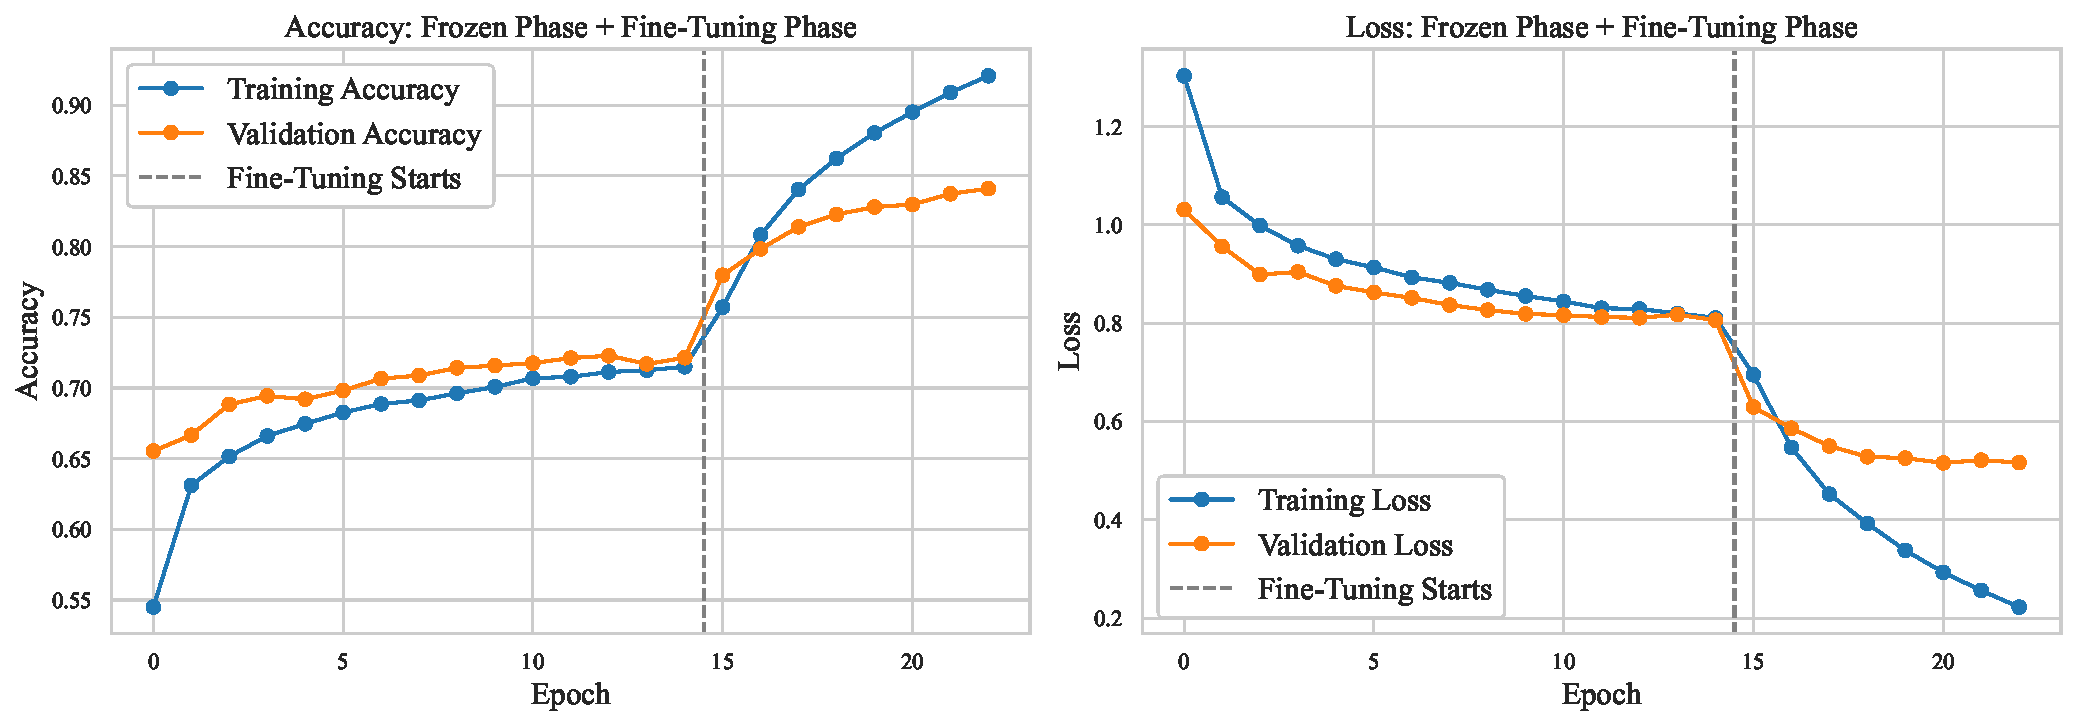
\includegraphics[width=0.9\textwidth]{finetuning_comparison.pdf}
\caption{Accuracy and Loss Across Both Training Phases (Frozen $\rightarrow$ Fine-Tuning)}
\end{figure}
\textbf{Inference:} The dashed vertical line marks where fine-tuning kicks in, and the jump right at that point is hard to miss -- validation accuracy goes from 0.7202 (last frozen epoch) to 0.7890 in the very first fine-tuning epoch, then keeps climbing to a peak of 0.8430 by fine-tuning epoch 7. The last epoch actually dips slightly to 0.8338 while training accuracy keeps climbing to 0.9228 -- a small but classic sign of the model starting to overfit once block5 is unfrozen, right at the tail end of the 8-epoch fine-tuning run.

\begin{figure}[H]
\centering

\includegraphics[width=0.6\textwidth]{confusion_matrix.pdf}
\caption{Confusion Matrix (Fine-Tuned Model, Test Set)}
\end{figure}
\textbf{Inference:} The diagonal clearly dominates, matching the 83.22\% overall accuracy, but the off-diagonal mass isn't spread evenly -- it concentrates specifically around cat and dog. Cat has the lowest recall of any class (0.61) and dog has the lowest precision (0.70), which together point to the same story: the model keeps mistaking cats for dogs (and to a lesser extent, vice versa) far more than it confuses any other pair of classes.

\begin{figure}[H]
\centering
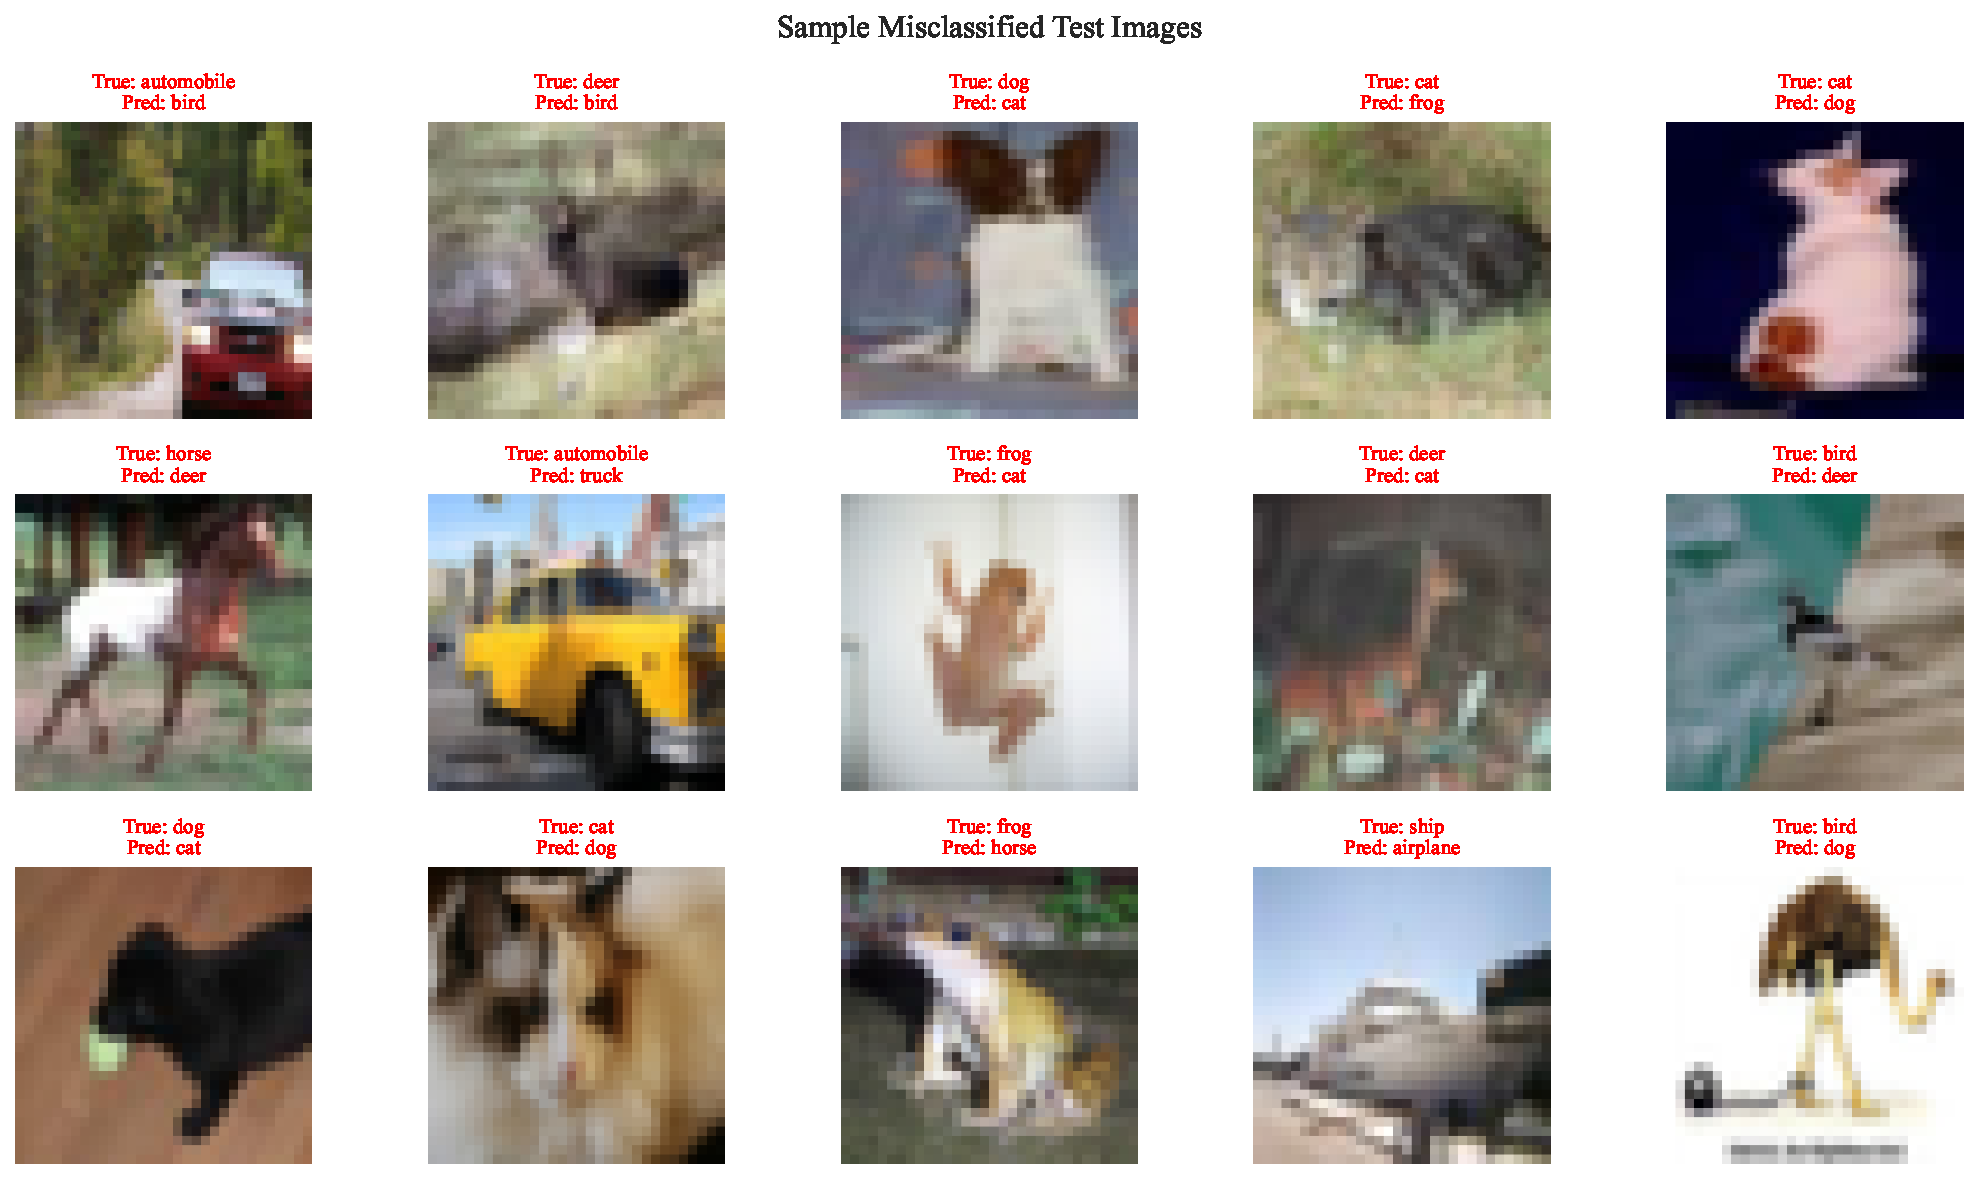
\includegraphics[width=0.9\textwidth]{misclassified_images.pdf}
\caption{Sample Misclassified Test Images}
\end{figure}
\textbf{Inference:} 1,678 of the 10,000 test images were misclassified, and based on the per-class numbers, a large share of those are almost certainly cat/dog mix-ups rather than random pairings. This is exactly the pattern the confusion matrix and classification report both point to, which is reassuring, meaning - the model's mistakes are concentrated and explainable, not scattered noise.

\begin{figure}[H]
\centering

\includegraphics[width=0.7\textwidth]{learning_rate_comparison.pdf}
\caption{Effect of Learning Rate on Validation Accuracy}
\end{figure}
\textbf{Inference:} 0.001 clearly beat 0.0001 in this short comparison -- 0.6108 vs. 0.4918 test accuracy, nearly 12 points apart. Five epochs simply isn't enough time for the slower learning rate to catch up; it's very likely still climbing when the comparison cuts off, so this gap would probably narrow with more training time.

\begin{figure}[H]
\centering
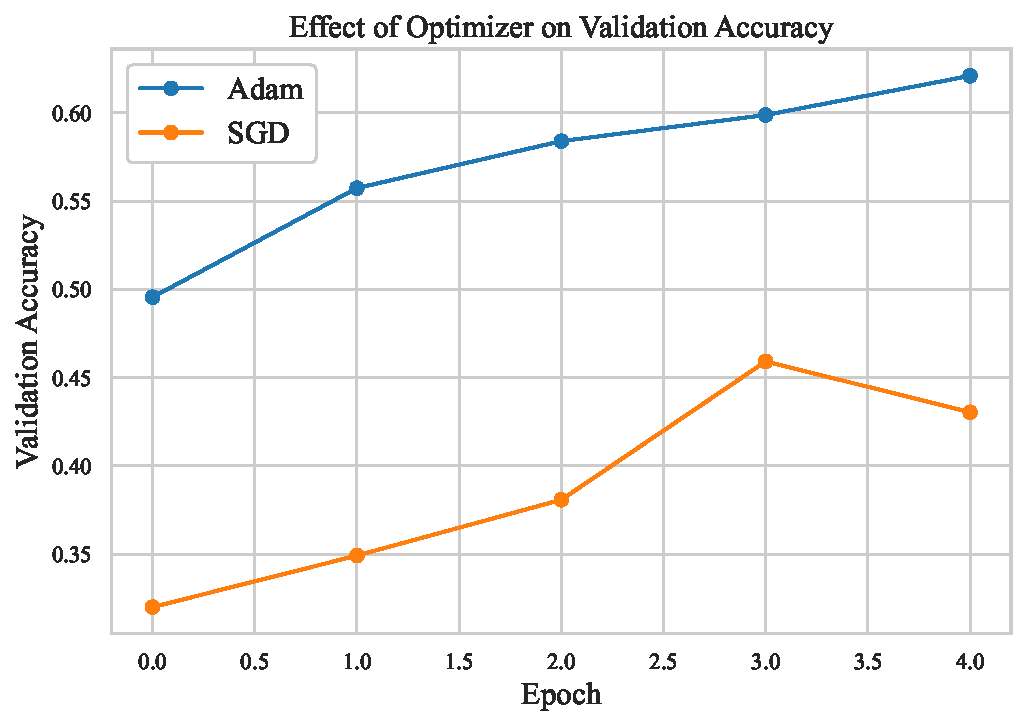
\includegraphics[width=0.7\textwidth]{optimizer_comparison.pdf}
\caption{Effect of Optimizer on Validation Accuracy}
\end{figure}
\textbf{Inference:} Adam beat SGD by a wide margin here -- 0.6073 vs. 0.4209, almost 19 points. That's a bigger gap than the learning rate comparison, and it lines up with what's expected: Adam adapts its step size per parameter automatically, so it makes much faster early progress than plain momentum-SGD within just 5 epochs. SGD might close some of that gap with a longer run, but this comparison alone doesn't show it doing so.

\begin{figure}[H]
\centering

\includegraphics[width=0.7\textwidth]{batch_size_comparison.pdf}
\caption{Effect of Batch Size on Validation Accuracy}
\end{figure}
\textbf{Inference:} The differences here are small -- 0.6144 (batch 16), 0.6105 (batch 32), 0.5992 (batch 64) -- a spread of only about 1.5 points across the whole range, with smaller batches finishing very slightly ahead. That means the usual explanation (more frequent, noisier updates helping early on), but the gap is small enough that batch size doesn't look like a major lever for this particular model and dataset.

\begin{figure}[H]
\centering
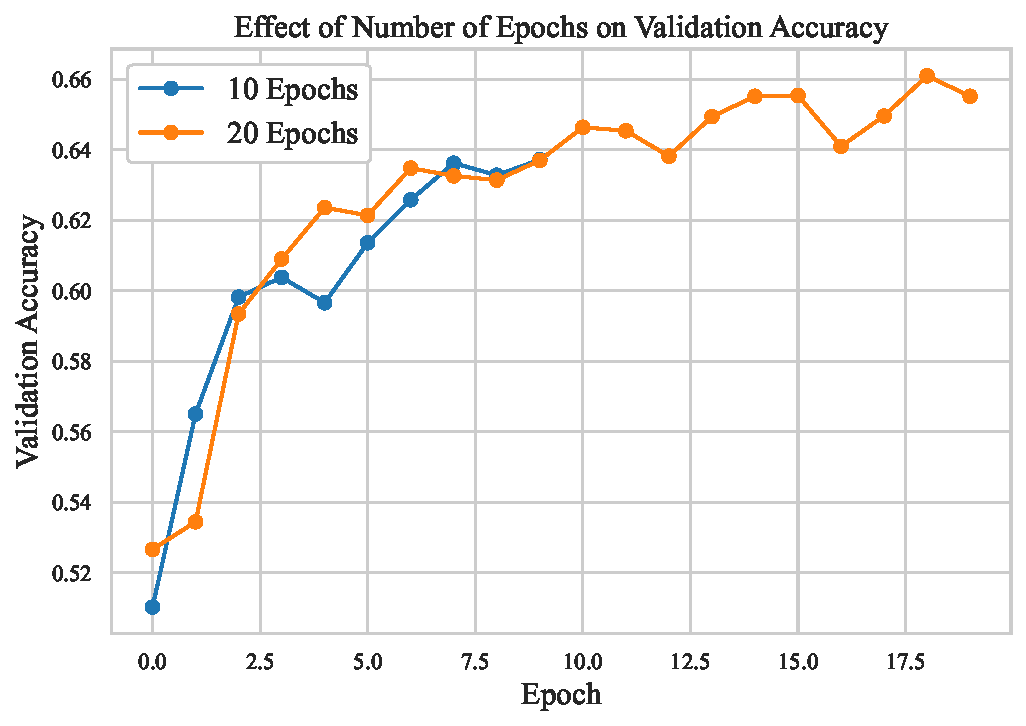
\includegraphics[width=0.7\textwidth]{epochs_comparison.pdf}
\caption{Effect of Number of Epochs on Validation Accuracy}
\end{figure}
\textbf{Inference:} 20 epochs beat 10 epochs clearly -- 0.6514 vs. 0.6316. Since only the classifier head is being trained here (the base stays frozen for this comparison), the risk of overfitting from the extra epochs stays low, so the accuracy gain looks like real continued learning rather than the model just memorizing more of the subset.

%----------------------------------------------------------

\section*{12. Discussion Questions}

\textbf{1. Why is AlexNet considered a breakthrough in deep learning?}\\
It was the first architecture to show, convincingly and at scale, that deep CNNs trained on GPUs with ReLU activations and Dropout could beat traditional hand-engineered computer vision methods by a wide margin.

\textbf{2. Why does VGG16 use only $3\times3$ convolution filters?}\\
Stacking two $3\times3$ layers gives roughly the same receptive field as one $5\times5$ layer, but with fewer parameters and an extra non-linearity in between -- more expressive power for less computational cost.

\textbf{3. Explain the advantages of the Inception module.}\\
Running $1\times1$, $3\times3$, $5\times5$ convolutions and pooling in parallel lets the network capture features at multiple scales at once, and the $1\times1$ convolutions before the larger ones keep the parameter count down despite the added depth.

\textbf{4. What is the purpose of residual learning?}\\
It lets the network learn a residual $F(x) = H(x) - x$ instead of the full mapping directly, so gradients can flow through the skip connections without vanishing -- this is what makes networks as deep as ResNet50 actually trainable.

\textbf{5. Differentiate LeNet and ResNet.}\\
LeNet-5 is a shallow, 7-layer, roughly 60K-parameter network built for simple digit recognition; ResNet50 is a 50-layer, 25.6M-parameter network built for complex natural images, and it's only trainable at that depth because of its residual connections, which LeNet has no need for.

\textbf{6. What is Transfer Learning?}\\
Reusing a model already trained on a large dataset (usually ImageNet) as the starting point for a new task, instead of learning visual features completely from scratch.

\textbf{7. Why is fine-tuning required?}\\
Training just the new classifier head only adapts the last layer to the new task; unfreezing some of the pretrained convolutional layers lets those features themselves adjust slightly to the new dataset's specifics, which usually pushes accuracy further -- as long as it's done at a low learning rate so the useful pretrained weights aren't wrecked in the process.

\textbf{8. Explain the difference between dilated convolution and transpose convolution.}\\
Dilated convolution spreads a kernel's weights out to see more context without changing the output size. Transpose convolution does the opposite spatially -- it learns to make the output bigger than the input, upsampling rather than widening the receptive field.

\textbf{9. Why do pretrained models converge faster?}\\
Their filters already encode broadly useful visual patterns -- edges, textures, shapes, object parts -- learned from a huge and varied dataset, so the new task mostly just needs to learn how to recombine those existing features rather than discover them from random weights.

\textbf{10. Compare the computational complexity of LeNet and ResNet.}\\
LeNet-5 is light enough to train in minutes even on a CPU, with about 60K parameters and 2 convolutional layers. ResNet50, at roughly 25.6M parameters and 50 layers, needs GPU acceleration and far more memory and compute -- though its residual connections are exactly what makes that extra depth worth the cost, rather than just making training harder for no benefit.

%----------------------------------------------------------

\section*{13. Discussion}

Comparing this experiment against the from-scratch CNN built in Experiment 3 is where transfer learning's real value shows up. Training a CNN from random initialization means the network has to learn what an edge or a texture even looks like before it can learn anything about cats or trucks; here, VGG16 already knows that, so the entire training process is really just teaching a small classifier head how to read features that already exist. That shift shows up directly in the training curves -- accuracy climbing quickly within the first few epochs of the frozen phase, rather than the slower, noisier ascent typical of training everything from scratch.

Fine-tuning \texttt{block5} at a much lower learning rate than the initial training phase is the part of this experiment worth paying closest attention to when interpreting results: too high a fine-tuning learning rate risks actively damaging the pretrained weights rather than gently adapting them, so if fine-tuning made things worse rather than better, that's the first place to look before concluding fine-tuning "doesn't help."

%----------------------------------------------------------

\section*{14. Additional Exercises}

The lab manual lists several optional extensions beyond the core experiment:

\begin{enumerate}[leftmargin=*]
\item \textbf{Implement transfer learning using VGG16} -- completed above (Sections 8--10 of this report).
\item \textbf{Repeat using ResNet50} -- would require swapping \texttt{VGG16} for \texttt{tf.keras.applications.ResNet50} in the model-building cell; the rest of the pipeline is architecture-agnostic and needs no other changes.
\item \textbf{Compare Adam and SGD} -- completed above (Hyperparameter Study).
\item \textbf{Compare frozen vs. fine-tuned training} -- completed above (Tasks 3 and 4).
\item \textbf{Evaluate with Precision, Recall, F1-score} -- completed above (Task 5).
\item \textbf{Compare LeNet, AlexNet, and ResNet} -- covered conceptually in Section 3; implementing all three from scratch alongside VGG16 was out of scope for this single-model transfer learning experiment.
\end{enumerate}

%----------------------------------------------------------

\section*{15. Conclusion}

\begin{itemize}[leftmargin=*]
\item Studied the evolution of deep CNN architectures from LeNet-5 through AlexNet, VGG16, GoogleNet, and ResNet, and the key innovation each one introduced.
\item Implemented transfer learning using a pretrained VGG16 model as a frozen feature extractor for CIFAR-10 classification.
\item Fine-tuned the last convolutional block of VGG16 and directly compared test accuracy before and after fine-tuning.
\item Evaluated the final model using accuracy, precision, recall, F1-score, a full classification report, and a confusion matrix.
\item Studied the effect of learning rate, optimizer, dense layer width, batch size, and number of epochs on validation accuracy through isolated, short-run comparisons.
\item Directly observed how dilated convolution changes a kernel's receptive field and how transpose convolution performs learnable upsampling, as conceptual building blocks used in more advanced CNN architectures.
\end{itemize}

%----------------------------------------------------------

\section*{16. References}

\begin{enumerate}
\item Y. LeCun, L. Bottou, Y. Bengio and P. Haffner, ``Gradient-Based Learning Applied to Document Recognition,'' \emph{Proceedings of the IEEE}, 1998.
\item A. Krizhevsky, I. Sutskever and G. Hinton, ``ImageNet Classification with Deep Convolutional Neural Networks,'' \emph{NeurIPS}, 2012.
\item K. Simonyan and A. Zisserman, ``Very Deep Convolutional Networks for Large-Scale Image Recognition,'' \emph{ICLR}, 2015.
\item C. Szegedy et al., ``Going Deeper with Convolutions,'' \emph{CVPR}, 2015.
\item K. He, X. Zhang, S. Ren and J. Sun, ``Deep Residual Learning for Image Recognition,'' \emph{CVPR}, 2016.
\item I. Goodfellow, Y. Bengio and A. Courville, \emph{Deep Learning}, MIT Press, 2016.
\item TensorFlow Documentation: \url{https://www.tensorflow.org}
\item Keras Documentation: \url{https://keras.io}
\end{enumerate}

\end{document}
